%; whizzy chapter
% -initex iniptex -latex platex -format platex -bibtex jbibtex -fmt fmt
% 以上 whizzytex を使用する場合の設定。

%     Kansai Debian Meeting resources
%     Copyright (C) 2007 Takaya Yamashita
%     Thank you for Tokyo Debian Meeting resources

%     This program is free software; you can redistribute it and/or modify
%     it under the terms of the GNU General Public License as published by
%     the Free Software Foundation; either version 2 of the License, or
%     (at your option) any later version.

%     This program is distributed in the hope that it will be useful,
%     but WITHOUT ANY WARRANTY; without even the implied warranty of
%     MERCHANTABILITY or FITNESS FOR A PARTICULAR PURPOSE.  See the
%     GNU General Public License for more details.

%     You should have received a copy of the GNU General Public License
%     along with this program; if not, write to the Free Software
%     Foundation, Inc., 51 Franklin St, Fifth Floor, Boston, MA  02110-1301 USA

%  preview (shell-command (concat "evince " (replace-regexp-in-string "tex$" "pdf"(buffer-file-name)) "&"))
% 画像ファイルを処理するためにはebbを利用してboundingboxを作成。
%(shell-command "cd image200708; ebb *.png")

%%ここからヘッダ開始。

\documentclass[mingoth,a4paper]{jsarticle}
\usepackage{kansaimonthlyreport}
\usepackage[dvips]{xy}
\usepackage{ascmac}

% 日付を定義する、毎月変わります。
\newcommand{\debmtgyear}{2010}
\newcommand{\debmtgdate}{27}
\newcommand{\debmtgmonth}{06}
\newcommand{\debmtgnumber}{36}

\begin{document}

\begin{titlepage}

% 毎月変更する部分、本文の末尾も修正することをわすれずに

 第\debmtgnumber{}回 関西 Debian 勉強会資料

\vspace{2cm}

\begin{center}
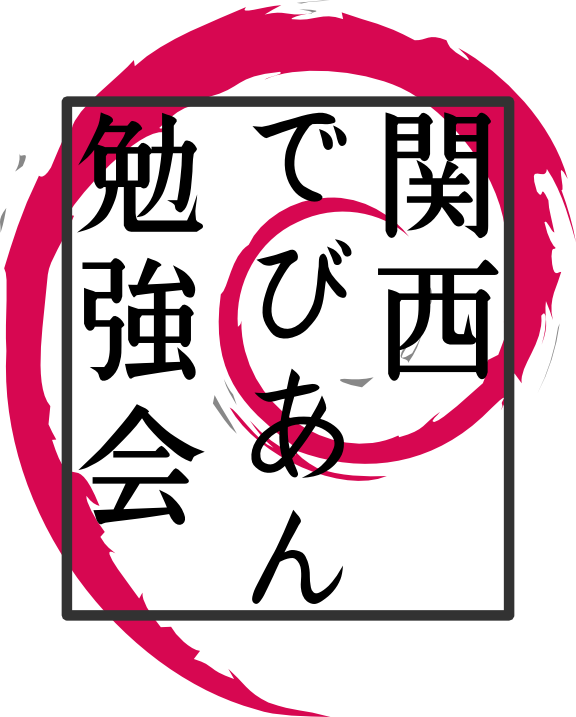
\includegraphics{image200802/kansaidebianlogo.png}
\end{center}

\begin{flushright}
\hfill{}関西 Debian 勉強会担当者 佐々木・倉敷・のがた \\
\hfill{}\debmtgyear{}年\debmtgmonth{}月\debmtgdate{}日
\end{flushright}

\thispagestyle{empty}
\end{titlepage}

\dancersection{Introduction}{Debian JP}

\subsection*{}%ロゴ用のスペース稼ぎ
 
関西 Debian 勉強会はDebian GNU/Linux のさまざまなトピック(新しいパッケー
ジ、Debian 特有の機能の仕組、Debian 界隈で起こった出来事、などなど)に
ついて話し合う会です。

目的として次の三つを考えています。
\begin{itemize}
      \item MLや掲示板ではなく、直接顔を合わせる事での情報交換の促進
      \item 定期的に集まれる場所
      \item 資料の作成
\end{itemize}

それでは、楽しい一時をお楽しみ下さい。

\clearpage

\begin{minipage}[b]{0.2\hsize}
 {\rotatebox{90}{\fontsize{80}{80}
{\gt 関西 Debian 勉強会}}}
\end{minipage}
\begin{minipage}[b]{0.8\hsize}
\hrule
\vspace{2mm}
\hrule
\setcounter{tocdepth}{1}
\tableofcontents
\vspace{2mm}
\hrule
\end{minipage}

\dancersection{最近のDebian関係のイベント報告}{Debian JP}

\subsection{前回の関西Debian勉強会}

前回の関西Debian勉強会は, 5 月 23 日に大阪港区民センターで行なわれました。
Ubuntu Japanese Team のあわしろいくやさんによる「Debian ユーザのための Ubuntu 入門」とのがたじゅんさんによる「次期リリースの Squeeze を見てみよう」でした。
%
リリースされたばかりの Lucid Lynx 入門が目玉でした。いくやさんのトークも
好調で、オフレコ話あり、Debian との差異ネタありでいい感じの盛り上がりを
見せていたと思います。

続いて、お約束通りにフリーズの遅れている squeeze について、のがたさんに
現状をまとめてもらいました。特に日本語まわりで課題が残っている squeeze、
リリースまで目が離せませんね。

\subsection{第 65 回東京 Debian 勉強会}

6月19日に第65回東京エリアDebian勉強会が開催されました。

内容はOSC北海道直前ということで、岩松さんによるDebian GNU/kFreeBSDの話と、
荒木さんによる「あなたはどっち?クラウドでDebian, Debianでクラウド」という
Debianでクラウドの話をされたそうです。

Debianでクラウド話の中では、今回、倉敷さんが発表するpuppetの話題も出たそ
うで興味深いですね。\footnote{あなたはどっち? クラウドでDebian // Debian
でクラウド / 荒木靖宏 -
\url{http://www.slideshare.net/ar\_maniacs/debian-debian} }


\dancersection{事前課題}{佐々木洋平}

今回はパッケージ作成にまつわる以下の事前課題を設定しました
\footnote{%
これまでと比べて思いっきりハードルを上げてしまったためか、
参加登録者が少ない気がしますが...}。
\begin{quote}
    \begin{screen}
        \begin{description}
              \item [deb パッケージ(野良含む)を作成している方] \\
            お手元のパッケージのどれか 1 つを source format 3.0、cdbs
            or debhelper 7 に移行して下さい。 提出事前課題としては、その
            感想をお願いします。 また、発表者宛に *debian.tar.gz を添付
            して下されば幸いです(その際には勉強会登録システムでの参加者
            名を明記して下さい)。
              \item [deb パッケージを作成していない方] \\
            パッケージ作成環境を一通り用意して来て欲しいので、お手元で
            適当なパッケージ(例えば GNU Hello)などを作成してきて下さ
            い。 提出事前課題としては、その感想をお願いします。
        \end{description}
    \end{screen}
\end{quote}

参加者の皆さんによる回答は以下の通りです。

\begin{prework}{ 佐々木洋平 }

    unstable の howm、rail パッケージの作成には debhelper
    7.0、rttools、rabbit パッケージの作成には CDBS + ruby-pkg-tools を
    使って rules を書きました。  ruby 関連について
    は setup.rb、install.rb、extconf.rb と install に使用するscript が
    分かれているので debhelper より CDBS + ruby-pkg-tools の方が楽です
    ね。 gem だと Rakefile になるので、debhelper
    7.0 用にdh\_rubygems(仮) を作成するなら Rake を探すようにすれば良い
    かな、と妄想しました。

\end{prework}

\begin{prework}{ 山田 洋平 }

    deb パッケージを作成していないほうです。
    Squeeze の hello および hello-debhelper と、
    「佐々木流」の資料を参考にしたら何とか作成できました。
    ですがもう少し中身を理解して作業したいです。
    
\end{prework}



\begin{prework}{ 西山和広 }

    cdbs を使ったパッケージはいくつか作ったことがあったので、source
    format 3.0 (quilt)で chkbuild の deb を作ってみまし
    た。\url{http://chkbuild.deb.n-z.jp/} で公開しています。cdbs と違っ
    て debian/rules に include がないので、DEB\_UPDATE\_RCD\_PARAMSなど
    を指定したくなった場合どうするのかが気になりましたが、今回は必要な
    かったのでそこまでは調べませんでした
    \footnote{%
      DEB\_UPDATE\_RCD\_PARAMS の場合は dh\_installinit を override
      します(佐々木)}。

\end{prework}



\begin{prework}{ かわだてつたろう }

GNU Hello でパッケージを作成。
単一のソースから単一のパッケージを作成するなら debhelper と debuild ですんなりとできるんだなぁと。
手間取ったところ:
\begin{itemize}
      \item lintian のエラー(package-contains-info-dir-file)
      \item pbuilder で basetgz 作成が何度も失敗
    \footnote{丁度 dennou-q のミラー障害時期に当たりましたかね?(佐々木)}
      \item piuparts での Broken symlinks で失敗
    \footnote{piuparts の Broken symlinks は鬼門ですね。
      多くの場合「オレの所為じゃねーよ」と叫びたくなります。}
\end{itemize}

\end{prework}



\begin{prework}{ 古川竜雄 }

    私はdebパッケージを作成していないので、課題どおりGNU Helloをパッケー
    ジ化してみました。参考書はmaint-guide-jaです。記述が古かったこ
    と、dh-makeが作るテンプレートのStandards-Versionが3.7.3なのに対し
    てLintianが3.8.0を要求(?)したことなどの問題を除けば、参考書の通りす
    んなりとできました。感想ですが、私はよくできていると思います。作業
    はめんどくさかったのですが、その原因は「ちゃんとしたパッケージを作
    る」ことにあり、これは必須のことです。そのめんどくささをツールでで
    きるだけ軽減するよう工夫されています。特に問題は感じませんでした。
    どう「進化」しているのか楽しみです!!

\end{prework}

\begin{prework}{ 榎真治 }

(回答なし)

\end{prework}

\begin{prework}{ lurdan }

    \begin{description}
          \item[source format 3.0] \\
        debian/ への変更が patches に入るのはまだしっくりきません%
        \footnote{%
          パッケージ作成の時に upstream へのソース変更が入ってい
          て、clean で変更が元に戻ってないのでは?(佐々木) }。
          \item[debhelper7] \\
        upstream がまともな Makefile を用意してくれてる場合は幸せになれ
        そうです。
    \end{description}
\end{prework}
\begin{prework}{ ”まさ”こと”甲斐正三”です }

(回答なし)

\end{prework}

\begin{prework}{ IPv6waterstar }
パラメータとエラーに悩まされた。以下、「入門 Debianパッケージ」を参照にしながら、時系列に今の状態を記す。
\begin{itemize}
      \item GNU Helloをダウンロード
      \item tar xvfz hello-2.6.tar.gzで解凍
      \item dh\_make --single --copyright=gplでdebinaディレクトリを作ろうとする
    も作ることができず、エラーを参照し、dh\_make --createorig --single
    --copyright=gplに修正し、debianディレクトリを作成。
      \item 「入門 Debianパッケージ」を参照し各ファイルを修正。
      \item debuild -uc -usをするも、debパッケージ作成されず、エラーを参照し、
    debuild -d -uc -usでパッケージを作成。エラー多し。
\end{itemize}
\end{prework}

\begin{prework}{ のがたじゅん }

すみません。最近の流れについてきてないので「deb パッケージを作成していな
い方」コースを選んでしまいました。GNU Helloのdebian/rulesを見ると、ごりご
り手で書いてるので、こういう方法もアリなんだと思いました。

\end{prework}
\begin{prework}{ 山下康成 }

パス。廊下で立ってます。ハイ

\end{prework}


\dancersection{dh {\normalsize $\sim$source format 3.0, the magic debhelper rules$\sim$}}{佐々木洋平}

次期安定版 6.0(squeeze)での RELEASE GOALS の一つに「new source package format support」があります\footnote{\url{http://release.debian.org/squeeze/goals.txt}}。
ここでの「new source package format」が {\bf source format 3.0} です。
\vspace{1em}

{\tt debhelper} は deb パッケージの構築を補助する様々なツール群です%
\footnote{%
deb パッケージそのものは {\tt debhelper} 無しでも作成できますが、
普通は {\tt debhelper} を使います。}。
多くのパッケージでは {\tt debhelper} の呼び出しはテンプレ化されているので
共通している {\tt debhelper} の呼び出しを隠蔽し
パッケージ作成のルール(debian/rules)を簡単にするのが
{\tt dh}(コマンド)と {\tt CDBS}(Makefile のルールセット)です。
\vspace{1em}

ここでは source format 3.0, dh, CDBS についてお話しします。
ちなみに、
告知タイトルに「深追い」とか「CDBS 2.0」とかいう文字列があった気がしますが
気にしないで下さい。

\subsection{source format 1.0 $\to$ 3.0 }

\subsubsection{1.0 の問題点}

source format 3.0 の前に、
これまでの source format 1.0 について簡単に復習しましょう。debian のソースパッケージは主に以下の構成物からなります:
\begin{quote}
    \begin{screen}
        \begin{description}
              \item[.orig.tar.gz]  \\
            オリジナルのソース一式
              \item[.dsc] \\
            パッケージの情報(パッケージの説明、メンテナ、ファイルのハッシュなど)
              \item[.diff.gz] \\
            バイナリパッケージをビルドするための変更点。
            Debian 固有のパッケージの場合には存在しない。
        \end{description}
    \end{screen}
\end{quote}

さて, このソースフォーマットの構成には, 以下の問題点があります:
\begin{enumerate}
      \item アーカイブの圧縮形式として .gz  しか使えない。
      \item upstream のソースが複数のアーカイブから構成される場合が面倒。
      \item パッケージメンテナの作成したパッチが全部単一のファイルにま
    とめられており、混然としている。
      \item diff で表現されるので(画像などの)バイナリが置きにくい。
\end{enumerate}

source format 1.0 の場合、これらの問題点は, だいたい以下の様に解決していました:
\begin{quote}
    \begin{description}
          \item[1. アーカイブの圧縮形式として .gz しか使えない。]  \\
        % 
        例えば upstream が bzip2 で配布されている場合でも gzip で圧縮しなお
        す、 もしくは tarball in tarball \footnote{%
          .orig.tar.gz を展開するとディレクトリ内にupstream の bzip2 が配置
          される。ビルドする際に tar を展開してからビルドする} などの形式に
        する、などです。
        % 
        後述の CDBS を使用する場合には tarball in tarball 用のルールとして
        {\tt tarball.mk} が用意されています。
        % 
           \item[%
        2. upstream のソースが複数のアーカイブから構成される場合が面倒。] \\
        % 
        前述の tarball in tarball で対応しています。
        % 
          \item[3. パッケージメンテナの作成したパッチが全部単一の patch に。]
         \\
        % 
        {\tt diff.gz} は {\tt debian} 以下のファイルが{\bf 全て}単一の
        ファイルになっています。{\tt debian/control} や 
        {\tt debian/rules} だけではなく、upstream のソースへのパッチも全て
        一つのファイルになっています。
        % 
        そこで、upstream のソースへのパッチは {\tt debian/patches} 以下に
        意味のある単位で分割して配置し、パッケージ作成の際に
        パッチの apply/unapply を行なうことにしています。
        % 
        このためのツールとしては{\tt dpatch} や
        {\tt quilt}
        \footnote{%
          こう書くと語弊があるかもしれませんが、
          {\tt quilt}は Debian 固有のツール{\bf ではありません}。
        %
          一方で dpatch は
          「patch maintenance system for Debian source packages」と
          あるように Debian 固有のツールです。
        }
        があります。
        % 
        また、CDBS にはパッチの apply/unapply をするためのルールとして
        {\tt patchsys-quilt.mk, dpatch.mk, simple-patchsys.mk}
        が用意されていますし、
        dh には{\tt --with quilt} というオプションが用意されています。
        % 
        ちなみに、
        各パッチの先頭にその意図を記述するタグを追加しておくことが推奨
        されています
        \footnote{\url{http://dep.debian.net/deps/dep3/} 
          面倒なので佐々木はサボリがちです。すいません。}。
        % 
          \item[4. diff で表現されるので(画像などの)バイナリが置きにくい。] \\
        uuencode/uudecode で diff が取れる形式にしておくなどして
         対応します。
    \end{description}
\end{quote}

というわけで、これまでの source format でも問題点について対応はできます。
しかしながら、
こういった特殊な操作を行なうことなく
問題点を解決するための新たなフォーマットとして、新たに
{\tt 3.0 (quilt)} と {\tt 3.0 (native)} が制定されました%
\footnote{%
  \url{http://wiki.debian.org/Projects/DebSrc3.0} 
  ちなみに 2.0 はどういう状況知りません. だれかご存知ですか?
}。

\subsubsection{3.0(quilt) と 3.0(native)}

{\tt 3.0 (quilt)} は以下のファイル群で構成されます:
\begin{quote}
    \begin{screen}
        \begin{description}
              \item[{\tt .orig.tar}.{\it ext}]  \\
            upstream のソース。複数のソースからなる場合には基本となるソースに
            この名前をつける。{\it ext} は圧縮の拡張子であり、
            gz, bz2, lzma, xz が使用可能。
            % 
              \item[{\tt .orig}{\it -component1}{\tt .tar.}{\it ext}] \\
            upstream が複数のソースから構成される場合に作成する。
            % 
            {\it -componet} はソースの名前に対応してメンテナが適宜名付ける。
              \item[{\tt .debian.tar.}{\it ext}] \\
            {\tt debian} ディレクトリの中身。
            {\it ext} は圧縮の拡張子であり、
            gz, bz2, lzma, xz が使用可能。
            %
            1.0 の {\tt diff.gz} から
            {\tt .tar.}{\it ext} になり、全てが混在した単一のパッチでは
            なくなった。
            % 
              \item[{\tt .dsc}]  \\
          パッケージに関する情報。
        \end{description}
    \end{screen}
\end{quote}
また {\tt 3.0 (native)} は 1.0 での Debian 固有パッケージに対応しており、
{\tt .orig.tar.}{\it ext} と {\tt .dch} ファイルからなります。

%
これらの変更により 1.0 での問題点は以下の様に解決されました。
\begin{enumerate}
      \item アーカイブの圧縮形式として .gz しか使えない。\\
    $\to$ .gzip, bzip2, lzma, xz を使用できるようになりました。
    %
      \item upstream のソースが複数のアーカイブから構成される場合が面倒。\\
    $\to$ {\tt .orig}{\it -component}{\tt .tar}{\it .ext} により
    複数のソースを使用できるようになりました。
    %
    これら{\tt .orig}{\it -component}{\tt .tar}{\it .ext} は
    ソースの展開時に {\tt compnent} というサブディレクトリに展開されます。
      \item パッケージメンテナの作成したパッチが全部単一のファイルに。
      \item diff で表現されるので(画像などの)バイナリが置きにくい。\\
    $\to$ {\tt .diff.gz} から {\tt .debian.tar.}{\it ext} になったので
    全てが混然となった状態は解消されており、バイナリも含めることができます。
    また、 {\tt debian/patches} に存在するパッチはソースパッケージの展開時に
    自動的に適用されるようになりました(これについては後述)。
\end{enumerate}

現在では、日々巨大化しつつある  Debian アーカイブのサイズを抑制するために
新規パッケージについては {\tt gzip} よりも {\tt xz} による圧縮が推奨されています。

\subsubsection{3.0 への移行}

さて source format 3.0 に以降するにはどうすれば良いでしょうか? 
複雑なパッケージでないならば、
\begin{commandline}
    % mkdir debian/source
    % echo '3.0 (quilt)' > debian/source/format
    % dch 'Switch to dpkg-source 3.0 (quilt) format' 
\end{commandline}
だけでです. 

これまでの diff.gz に upstream へのパッチが含まれている場合には、
先ずパッチを(意味のある単位に)分割し、
quilt で管理できるようにしておきましょう。
そうしない場合には分割されていないパッチは
{\tt debian/patches/debian-changes-<version>} という
patch にまとめられてしまいます\footnote{というわけです $>$ lurdan}。
また、
更新の度に{\tt debian-changes-<version>} というパッチが生成されてしまいます。
%
また quilt は -p1 のパッチしか扱えませんので rules 内で明示的に patch
-p0 とか patch -p2 としている場合や、 CDBS の simple-patchsys.mk を使用
している場合には -p1 で適用できるようにパッチを変更しておきます。

最後に debian/rules でのパッチに関する rules を消しておくことが推奨され
ています。dpkg ($>$=1.15.5.4) では dpkg-source によってソースを展開する
際にdebian/patches 以下のパッチが自動的に適用されることは既に述べました。
古い buildd、とくに lenny 向けの buildd ではソースを buildd chrootの外
で展開することがあるため, dpkg-source の段階でソースにパッチが適用され
ていない場合には不具合が生じます。
%
パッチを更新した場合には debuild を実行する前にパッチを全て適用しておき
ます。こうして debuild を実行すると、3.0 形式のソースパッケージが生成さ
れます。

ちなみに lenny の dpkg は既に 3.0 に対応しています。これ
はlenny で squeeze のソースパッケージを使用する場合(backports 等)に問題
にならないようにするためです。 また、現在は {\tt debian/source/format}
で source format のバージョンを指定していますが、将来的には全て新しい
source format へ移行される予定です。
\begin{center}
    {\tt ではお手元のソースを 3.0 へ移行してみましょう}    
\end{center}

\subsection{debian/rules の書き方}

CDBS, dh 以前の debhelper コマンド群を使用した {\tt debian/rules} は
一番簡単な場合でも、
例えば以下の様になります
\footnote{lenny で GNU Hello のパッケージを作成した場合です。
ページに収めるために先頭のコメントを削っています。}。
\begin{commandline}
#!/usr/bin/make -f
# -*- makefile -*-
# Sample debian/rules that uses debhelper.
# - snip -

# Uncomment this to turn on verbose mode.
#export DH_VERBOSE=1
 
# These are used for cross-compiling and for saving the configure script
# from having to guess our platform (since we know it already)
DEB_HOST_GNU_TYPE   ?= $(shell dpkg-architecture -qDEB_HOST_GNU_TYPE)
DEB_BUILD_GNU_TYPE  ?= $(shell dpkg-architecture -qDEB_BUILD_GNU_TYPE)
ifneq ($(DEB_HOST_GNU_TYPE),$(DEB_BUILD_GNU_TYPE))
CROSS= --build $(DEB_BUILD_GNU_TYPE) --host $(DEB_HOST_GNU_TYPE)
else
CROSS= --build $(DEB_BUILD_GNU_TYPE)
endif
config.status: configure
        dh_testdir
        # Add here commands to configure the package.
ifneq "$(wildcard /usr/share/misc/config.sub)'' "
        cp -f /usr/share/misc/config.sub config.sub
endif
ifneq ``$(wildcard /usr/share/misc/config.guess)" ""
        cp -f /usr/share/misc/config.guess config.guess
endif
        ./configure $(CROSS) --prefix=/usr --mandir=\$${prefix}/share/man --info
dir=\$${prefix}/share/info CFLAGS=''$(CFLAGS)" LDFLAGS="-Wl,-z,defs"


build: build-stamp

build-stamp:  config.status
        dh_testdir

        # Add here commands to compile the package.
        $(MAKE)
        #docbook-to-man debian/hello.sgml > hello.1

        touch $@

clean:
        dh_testdir
        dh_testroot
        rm -f build-stamp

        # Add here commands to clean up after the build process.
        [ ! -f Makefile ] || $(MAKE) distclean
        rm -f config.sub config.guess

        dh_clean

install: build
        dh_testdir
        dh_testroot
        dh_clean -k
        dh_installdirs

        # Add here commands to install the package into debian/hello.
        $(MAKE) DESTDIR=$(CURDIR)/debian/hello install

# Build architecture-independent files here.
binary-indep: build install
# We have nothing to do by default.

# Build architecture-dependent files here.
binary-arch: build install
        dh_testdir
        dh_testroot
        dh_installchangelogs ChangeLog
        dh_installdocs
        dh_installexamples
#       dh_install
#       dh_installmenu
#       dh_installdebconf
#       dh_installlogrotate
#       dh_installemacsen
#       dh_installpam
#       dh_installmime
#       dh_python
#       dh_installinit
#       dh_installcron
#       dh_installinfo
        dh_installman
        dh_link
        dh_strip
        dh_compress
        dh_fixperms
#       dh_perl
#       dh_makeshlibs
        dh_installdeb
        dh_shlibdeps
        dh_gencontrol
        dh_md5sums
        dh_builddeb

binary: binary-indep binary-arch
.PHONY: build clean binary-indep binary-arch binary install    
\end{commandline}
configure、make、 make install 以外にも随所に dh\_ から始まるコマンドが
呼び出されています。
%
この dh\_ から始まるコマンドが debhelper コマンド群です。
%
幾つかの例外を除いて dh\_* は適切なタイミングで呼び出すだけですので、
この呼び出しを隠蔽するだけで debian/rules は随分すっきりします。
CDBS, dh は異なる手法で dh\_* の呼び出しの隠蔽とルールセットの追加を
行なっています。

\subsubsection{CDBS}

CDBS については以前お話しました(2008年6月, 第 18 回関西Debian勉強会%
\footnote{\url{http://tokyodebian.alioth.debian.org/pdf/debianmeetingresume200810-kansai.pdf}})。{\tt debian/ruls} は Makefile ですので
\begin{itemize}
      \item Makefile の target を細分化。
      \item ソフトウェアやパッケージの状況に応じて、
    呼び出す target を class としてまとめる。
\end{itemize}
としています。

CDBS を利用した場合のビルドターゲットの流れについては例えば
杉浦さんの Web に良い絵が公開されています
(これは buildcore.mk + debhelper.mk を用いた場合です)。
\begin{figure}[h]
    \centering
    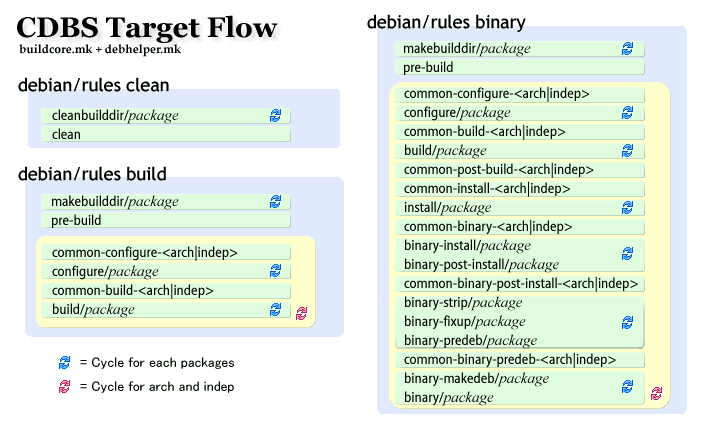
\includegraphics[width=0.7\textwidth]{./image201006/cdbs-targets.png}
    \caption{%
      CDBS Target flow:
      \url{http://sugi.nemui.org/doc/cdbs/cdbs-targets.png}}
    \label{fig:CDBSTargetFlow}
\end{figure}

CDBS を使った場合、先程の GNU Hello のルールは
\begin{commandline}
#!/usr/bin/make -f

include /usr/share/cdbs/1/rules/debhelper.mk
include /usr/share/cdbs/1/class/autotools.mk
\end{commandline}
となります。
以前書きましたが, %
いきなりコレだと今度は何をしているのかわからなくなりますね(笑)。

最初の include が dh\_* の呼び出しを設定する class, 
二つ目の include が autotools を使用するソースからパッケージを作成する場合の
class です。CDBS の詳細については本家のドキュメント\footnote{%
CDBS Documentation: \url{http://cdbs-doc.duckcorp.org/en/cdbs-doc.xhtml}}
が参考になるでしょう。
%
パッケージに付属のドキュメントではソースには実装されていて使えるのに
ドキュメント化されていない便利機能が多いです。
%
こういう場合は「ソース見れば良いじゃん」というのはまあ正論ではあります。%
実際、class のカスタマイズに使用する変数はソース冒頭に定義されてますし...。


\subsubsection{dh - debhelper command sequencer}

CDBS が make の target の細分化$\to$class 化という方向で dh\_* の呼び出
しを隠蔽し、Gnome、KDE といった統合環境や perl、python といった言語用
の class によって rules の作成を容易にしているのに対して、
dh のアプローチは以下の通りです:
\begin{itemize}
      \item debhelper の呼び出しは隠蔽したまま
      \item 
    パッケージ作成に使用するツール(autotools, make, MaikeMaker 等)
    の自動判定を行なう
\end{itemize}


例えば先程の GNU Hello の場合には
となります。
\begin{commandline}
#!/usr/bin/make -f

%:
        dh $@
\end{commandline}
...CDBS よりさらに簡潔になりました(笑)。

さて、これでは CDBS 以上にナニをしているのかわかりませんね。
実は dh コマンドには {\tt --no-act} というオプションが用意されています。
試しに rules を書き換えずに binary ターゲットを --no-act つきで
実行してみましょう。
\begin{commandline}
   uwabami@vmguest-lenny:~/Packages/hello-2.6$ dh binary --no-act
   dh_testdir
   dh_auto_configure
   dh_auto_build
   dh_auto_test
   dh_testroot
   dh_prep
   dh_installdirs
   dh_auto_install
   dh_install
   dh_installdocs
   dh_installchangelogs
   dh_installexamples
   dh_installman
   dh_installcatalogs
   dh_installcron
   dh_installdebconf
   dh_installcatalogs
   dh_installemacsen
   dh_installifupdown
   dh_installinfo
   dh_installinit
   dh_installmenu
   dh_installmime
   dh_installmodules
   dh_installlogcheck
   dh_installlogrotate
   dh_installpam
   dh_installppp
   dh_installudev
   dh_installwm
   dh_installxfonts
   dh_lintian
   dh_desktop
   dh_gconf
   dh_icons
   dh_perl
   dh_pysupport
   dh_scrollkeeper
   dh_usrlocal
   dh_link
   dh_compress
   dh_fixperms
   dh_strip
   dh_makeshlibs
   dh_shlibdeps
   dh_installdeb
   dh_gencontrol
   dh_md5sums
   dh_builddeb
\end{commandline}
と出力されます。CDBS と違って、ビルド時の流れを見る事ができます。
dh コマンドの肝は
\begin{center}
    {\tt dh\_auto\_}
\end{center}
で始まる 5 つのコマンドです。

何も設定しない場合には dh\_auto\_configure がパッケージの
ビルド時に使用するツールを判定します。この判定結果に基づき
auto\_build, auto\_test, auto\_install が実行されます。
自動判定結果は基本的に良くある GNU な設定になっており、
例えば configure 時の --prefix=/usr とか install 時の DESTDIRなどは
GNU のパッケージ用に設定されています(なので GNU Hello は設定が不要です)。

注意して欲しいのは configure や configure.ac をパースしているわけではないので
dh\_auto\_* は変数を自動設定をしているわけではない、という事です。
configure に対して Debian パッケージ用のフラグを適用したり、環境変数を追加
する場合には、適宜変数を設定してやったりする必要があります。
%
また、ソフトウェアによっては
ビルド時に configure, make, make install 以外の操作をする必要があったりします。
このための機能が dh の {\tt override} と {\tt before, after} です。

\subsubsection{実践! the magic debhelper rules}

例えば GNU Hello の configure オプションには
{\tt --with-gnu-ld} や {\tt --disable-nls} といったオプションがあります。
これらを configure 時に指定したい、と思ったらどうしたら良いでしょう?
この場合には dh\_auto\_configure の呼び出し時にオプションを与えるようにします。
例えば lenny の場合には {\tt --before, --after} を使用します。
\begin{commandline}
#!/usr/bin/make -f

%:
        dh $@

build: build-stamp
build-stamp:
        dh build --before configure
        dh_auto_configure -- --with-gnu-ld --disable-nls
        dh build --after configure
        touch build-stamp
\end{commandline}
squeeze/sid の dh には {\tt override} という機能が追加されており、
記述がさらに簡単になります%
\footnote{override は debhelper ($>$= 7.0.50) 以降の機能です。}。
\begin{commandline}
#!/usr/bin/make -f

%:
        dh $@

overide_dh_auto_configure:
        dh_auto_configure -- --with-gnu-ld --disable-nls
\end{commandline}
squeeze/sid 版の override の方が直感的にわかりやすいですね。 
また、squeeze/sid の dh コマンドは --no-act の際に override 
を表示してくれます。
\begin{commandline}
uwabami@vmguest-sid:~/Packages/hello-2.6$ dh binary --no-act
  dh_testdir
  debian/rules override_dh_auto_configure
  dh_auto_build
  dh_auto_test
  ...
\end{commandline}
override の詳細までは表示されませんが override されていること、
及び呼び出しの順番が参照できます\footnote{%
西山さんの DEB\_UPDATE\_RCD\_PARAMS の場合は
dh\_installinit を override すれば良いと思います.}。

以下では squeeze/sid の dh コマンドについて解説します。
残念ながら lenny の debhelper は若干古いですので、
sqeeze/sid の debhelper を導入しましょう。
%
dh コマンドの使い方については
Debconf9 での Joey Hess 御大による debhelper のプレゼン資料
\footnote{%
\url{http://joey.kitenet.net/talks/debhelper/debhelper-slides.pdf}}
が今の所一番まとまっている気がします。
御大のプレゼン資料に掲載されている
dh コマンドを利用した rules の例を以下に示します。
\begin{enumerate}
      \item 自動判定結果とは別のビルドツールを使用
    \begin{commandline}
#!/usr/bin/make -f

%:
    dh $@ --buildsystem perl_build
    \end{commandline}
      \item upstream のソースファイルがサブディレクトリ src にあり
    ビルドを make -C で別ディレクトリ(ここでは build)で実行
    \begin{commandline}
#!/usr/bin/make -f

%:
    dh $@ --sourcedirectory=src \
          --builddirectory=build
    \end{commandline}
      \item パッチ当てに quilt を使用して、
    configure にフラッグを指定、changelog として changelog.html
    を収録
    \begin{commandline}
#!/usr/bin/make -f

%:
    dh $@ --with quilt \
          --builddirectory obj \
          --sourcedirectory source 

override_dh_auto_configure:
    autoconf
    dh_auto_configure -- --with-sdl CC=/usr/bin/gcc-4.1

override_dh_installchangelogs:
    dh_installchangelos changelog.html
    \end{commandline}
 \end{enumerate}
などなど。

\subsection{debhelper vs CDBS vs dh }

Joey Hess 御大のプレゼン資料では
\begin{itemize}
      \item debhelper で設定可能な項目は 138
      \item CDBS で設定可能な項目は 138 + 153
      \item dh で設定可能な項目は 138 + 12
\end{itemize}
となっています。

御大は「私が比較するのは unfair だ」とおっしゃってますが、
rules の可読性/可変性は dh の方が圧倒的に優れていると思います。
特に、dh の一番嬉しい所は
--no-act による work frow が把握しやすいことでしょう。
また、Build-Depends が減る、というのは一つの利点かもしれません。

一方、CDBS は work flow は把握しにくいですけれど対応している
ビルドツールが多い事があげられます。
CDBS 本体には Make, SCons(Make の代替品), 
Perl, Python, Cmake, Ant,  Qmake, Gnome, KDE の class がありますし、
本体には収録されていませんが pkg-kde-tools, pkg-ruby-tools が提供されています。
これらの class を使用することで rules は共通化され非常に簡潔に記述できます。
dh の場合, 現時点で対応しているビルドツールは
\begin{commandline}
uwabami@vmguest-sid$ dh_auto_build --list
autoconf             GNU Autoconf (configure)
perl_makemaker       Perl ExtUtils::MakeMaker (Makefile.PL)
makefile             simple Makefile
python_distutils     Python Distutils (setup.py)
perl_build           Perl Module::Build (Build.PL)
cmake                CMake (CMakeLists.txt)
ant                  Ant (build.xml)
qmake                qmake (*.pro)
\end{commandline}
といった所です。


\begin{center}
    {\tt ではお手元のソースを CDBS or dh へ移行してみましょう. \\
    既に CDBS を使用している場合には dh で書きかえて見て下さい。}
\end{center}

最後に妄想など。
%
現在手元で dh\_ruby 関連を作成中です。
setup.rb, extconf.rb ができれば多分 CDBS とは別の選択肢になるだろう, と
思っています(あとは rake 用の build 拡張ができれば dh\_make\_gems の完成です)。
これについては...時間と紙面の都合で今日は載せられません。そのうち勉強会で
お話しします。
というわけで、「深追い」はタイトルに偽りアリ、ですね。すみません...{\tt Orz}

\dancersection{puppetに {\tt \textdollar HOME} を管理させてみよう}{倉敷悟}

今回は、皆さんの道具箱に入っていると便利な puppet というツールを
ご紹介します。

\subsection{はじめての糸繰り}

早速ですが、まずは動かしてみてもらおうと思います。lv をネタに使うので、
lv の設定を \textasciitilde /.lv に書いている人は、一旦適当に退避してください。

念の為、進む前に \textasciitilde /.lv が存在しないことを確認しておきましょう。

\subsubsection{実行サンプル}

なにはともあれ、puppet をインストールします。

puppet-el は、emacs でシンタックスハイライトさせるためのものなので、
emacs を使わない人はなくても OK ですが、なしでは割とやってられません。

\begin{commandline}
$ sudo aptitude install puppet puppet-el
$ emacs site.pp 
\end{commandline}

エディタが起動したら、site.pp には次のように入力してください。site.pp は
糸繰りの譜面、つまり設定ファイルです。なお、{\tt \#} はコメントなので無視して頂いて構いません。

\begin{commandline}
  # sudo が必要
  package { "lv":
    ensure => installed,
  }

  file { "/home/yourname/.lv":
    content => "-c",
  }
\end{commandline}

入力が終わったら、保存してコマンドに戻ります。では、いよいよ puppet に踊っ
てもらうことにします。
ネットに接続できるなら、aptitude purge lv してからでもいいでしょう。

\begin{commandline}
$ puppet site.pp
\end{commandline}

何が起きたか確認してみてください。予想通りすぎて、ちょっと拍子抜けかも知
れませんが……。

\newpage
\subsection{概要}

\subsubsection{用語の整理}

先に進む前に、用語の紹介だけしておきます。

site.pp に入力してもらった設定のことをマニフェストと呼び、ここに、必要な
リソースを宣言することで、puppet を操っていきます。

先ほど書いてもらったマニフェストでは、package と file がそれぞれ
リソースの宣言になります。
puppet が理解できるリソースはあらかじめ決まっていますが、自分で新しく
リソースを作ることもできます。

リソースの構成要素と、基本的な書式は次のようになります。区切りの記号に注意してください。

\begin{itemize}
 \item タイプ : リソースの種類
 \item タイトル : 「その」リソースの名前
 \item 属性 : 様々なパラメータ
\end{itemize}

\begin{commandline}
タイプ {
  "タイトル":
    属性 => 値,
    属性 => 値,
    ...
    属性 => 値;
  "タイトル":
    ...
}
\end{commandline}

\subsection{puppet の概要}

ここで一旦手を休めて、puppet そのものについて、もう少し説明しておきます。

puppet が何か、を一言でいえば、システム構成の管理ツールということになります。
普段、sudo を使ってやるような「パッケージ操作」「/etc 配下の設定変更」
「プロセスの起動停止」といった作業内容を、事前にレシピを書いておくことで、
puppet に任せることができます。

\subsubsection{構成}

puppet は、だいたい次のような構成で動きます。

\begin{itemize}
\item puppet : マニフェストを実行するコマンド
\item puppetd : puppetmasterd にマニフェストをリクエストして、それを実行するデーモン
\item puppetmasterd : マニフェストの束をもっていて、puppetd のリクエスト
      にあわせて適切に配布するデーモン
\end{itemize}

実は、puppet を使う場合は、puppetmasterd と puppetd の組み合わせで多数の
ホストを集中管理するのが普通だったりします。

ですが、今回はそれは一旦おいておいて、puppet コマンドを使ったお手軽な方
法をベースに進めていきますのでご承知置きください。

最後でもご紹介しますが、普通の構成についても既に山ほど記事や資料はあるので、
興味がある方はそちらをご参照頂ければと思います。

\newpage
\subsubsection{ディレクトリ配置}

puppet が使用するディレクトリですが、典型的にはこんな感じです。設定でど
うとでも変えられるので、配置されるものの種類がこんな感じなのだと思ってく
ださい。

実際のところ、puppet コマンドを使う場合は、/etc/puppet ではなくて
\textasciitilde /.puppet が主な作業場所として想定されます。

\begin{itemize}
 \item /etc/puppet/ : puppet 自体の動作設定ファイルが配置されます
 \item /etc/puppet/manifests : マニフェストが配置されます
 \item /etc/puppet/templates : テンプレートファイルが配置されます
 \item /etc/puppet/modules : puppet module が配置されます
 \item /var/lib/puppet : マニフェストのキャッシュや、SSL 証明書が配置さ
       れます
\end{itemize}

ここで、最初に作ったマニフェストを、\textasciitilde /.puppet/manifests に移動させておい
てください。puppet を実行した時点で、\textasciitilde /.puppet は作成されているはずです。


\subsection{設定を増やす}

では、実践に戻ります。lv だけでは寂しいので、他にもレシピを追加して
みることにします。ちょっと時間をとるので、自分的に必須なツールなど、
適当に書いてみてください。emacs でも screen でも何でも OK です。


\subsection{リソースの整理}

設定をどんどん追加していくと、site.pp にずらずらとリソースが並んで、
大変見通しが悪くなってきます。そこで、リソースをグルーピングすることにしましょう。

puppet で用意されているリソースのグルーピング方法には、ノード、クラス、
デファイン、モジュール、といったものがあります。

\subsubsection{ノード}

ノードは、ホストの fqdn と関連づけられるリソースのグループです。「この
fqdn のホストに、このリソースをまとめて反映しといて!」というイメージです。

実際の定義はこんな感じになります。

\begin{commandline}
node myhost01.localdomain {
  file {.....}
  service {.....}
}
\end{commandline}

node の中に書いた定義は、ホスト名が指定されたものと一致しているホストで
のみ有効になります。

emacs はマシン全部に入れるけど、wicd はデスクトップには要らないや、
みたいな使い分けが考えられます。

\subsubsection{クラス}

クラスは、ノード程具体的ではないのですが、「何となく関係しているリソースを
まとめて名前つけとこ!」というイメージのものです。
実際に使うときは、事前に定義した class をマニフェスト中で include する
必要があります。

実際の定義はこんな感じになります。

\begin{commandline}
class myconfig {
  file {.....}
  package {.....}
}

include myconfig
\end{commandline}

\subsubsection{デファイン}

デファインは、クラスと似ているのですが、引数を取れるところと、デファイン
で定義したリソースは複数回設定できるところが違っています。

実際の定義はこんな感じになります。

\begin{commandline}
define emacs::config ( $content, ){
  file { $name.el:
    content => $content,
  }
}

emacs::config { "howm":
  content => ”(require 'howm)"
}
\end{commandline}

個人的には、クラスを補完する目的で使うことが多いでしょうか。クラスとの比
較例でもよく使われますが、apache クラス (1回だけ登場) の補助で、デファイン
しておいた apache::vhost (複数回登場) を使う、などです。


\subsubsection{モジュール}

モジュールは、前述したノードやクラスとはちょっと位置付けが異なっていて、
マニフェストの書き方というよりは、ファイルの配置の仕方でグルーピングを
するものです。

基本的には、先に触れた puppetdir/modules の下に、ミニ puppet
設定ディレクトリを作ります。
よく使うので一応 fles と templates も書いていますが、モジュールと
しては少なくとも init.ppがあれば機能します。

\begin{commandline}
modules/
 モジュールの名前/
   manifests/
     init.pp
   files/
   templates/
\end{commandline}

一まとまりの大きな機能をモジュールとして構成しておいて、必要な場合だけ
読み込む、といったことができます。

また、自分が書いているマニフェストの中でも、独立性を高くして切り離すこと
ができるので、他の人とマニフェストを交換する場合に便利です。
github などで、モジュール個別のリポジトリが公開している人などもいて、
お手本としても役立ちます。

\subsection{モジュールの切り出し}

書いたマニフェストが充実してきたら、モジュールとして切り出すようにしたい
のですが、今回は時間もないので、充実していないながら一度切り出しを試して
みようと思います。

\subsubsection{lv モジュール}

では、一度 .puppet/modules に移動して、モジュールのためのディレクトリを
用意して、モジュールを作ってみましょう。

\begin{commandline}
mkdir -p ~/.puppet/modules/lv/manifests
emacs ~/.puppet/modules/lv/manifests/init.pp
\end{commandline}
 
\begin{commandline}
class lv {

ここに最初に書いた内容をコピー

}
\end{commandline}

site.pp に書いていた、同じ内容は消しておいてください。puppet では、同じ
名前をもったリソース宣言は重複としてエラーになります。

\subsubsection{モジュールの読み込み}

さて、設定を切り出したのはいいですが、さっきと同じように puppet コマンド
を実行しても、切り出した部分は動いてくれません。init.pp を直接引数にすれ
ば動かなくもないですが、設定が複雑になったり、複数のモジュールを使いたく
なったら破綻します。

puppet にモジュールを認識させるには、次のステップが必要です。

\begin{enumerate}
 \item puppet の設定 (modulepath) でモジュールの配置場所を教える
 \item site.pp からそのモジュールで定義したクラスを include する
\end{enumerate}

これを実現するため、site.pp に、include lv という一文を追加して、
こういうコマンドラインでもう一度実行してみましょう。

\begin{commandline}
puppet --modulepath ~/.puppet/modules ~/.puppet/manifests/site.pp
\end{commandline}

さて、無事に動いたでしょうか。

\subsubsection{切り出しで迷ったら}

愛情こめて育てた site.pp からモジュールを切り出そう、と思ったときに、
どういう名前でどの範囲を切り取るか、迷うことがあるかも知れません。

そんな時は、使おうとしている機能を提供するパッケージとモジュールを
対応づけるのがおすすめです。

すでに作った lv モジュールや、emacs モジュール、apache モジュール、
xmonad モジュール、platex モジュール……などと考えるわけです。

切り分けの単位としてわかりやすいことと、puppet が OS のパッケージ
システムとうまく連携してくれるために、後で複数のモジュールを組み合わせ
たくなった時にやりやすい、のがポイントです。

また、後で別の用途にそのモジュールを使い回すには……と考えながら作ると、
機能面でもいい具合に切り分けできるのではないかと思います。

\subsubsection{puppet-module ツールの紹介}

puppet を作っている puppetlabs という企業が、最近モジュール用の
リポジトリとして alioth のようなサイトをオープンしました。

\url{http://forge.puppetlabs.com/}

ブラウザでジャンル毎に公開されているモジュールを探したりできる
ようになっています。今はまだ登録されているモジュールの数が少ないですが、
そのうち充実してくれば、モジュールのカタログとして便利に使えるようになる
のではと思います。

このサイトと連動して、検索や取得 (その気があれば公開も) をするための
コマンドラインツールもあります。それが puppet-module です。

今のところ github からの取得になりますが、そのうち ruby 関連のメンテナ
がパッケージにするでしょう。

実際に使うとこんな感じです。

\begin{commandline}
puppet-module search [keyword]
\end{commandline}
で欲しいモジュールを探して、

\begin{commandline}
puppet-module install xx-yyy
\end{commandline}

でダウンロードしてきます。指定している xx-yyy ですが、forge での
名前空間は、xx (作者名)/yyy (モジュール名) となっていて、それを
指定します。自分の名前が頭につくので、モジュール名は他の人とかぶっても
大丈夫、ということですね。

注意が必要なのは、install とはいいながら、コマンドを実行したカレント
ディレクトリに展開するだけで、puppetdir/modules に自動で配置して
くれるわけではないところです。ダウンロードした後で、自分で移動させてください。

puppet-module には generate という機能もあり、モジュールの雛形を
作ってくれます。この場合も、forge の名前空間を指定する必要があるので、
使用例は次のようになります。

\begin{commandline}
$ bin/puppet-module generate lurdan-homedir
$ mv lurdan-homedir ~/.puppet/modules
$ cd lurdan-homedir
$ emacs manifests/init.pp
\end{commandline}

generate で作成されるディレクトリ構造はこんな感じになります。モジュール
としてフル機能が実装できるように、あれこれ気を利かせてくれている感じがし
ますね。

\begin{commandline} 
Modulefile
README
manifests/
files/
templates/
tests/
lib/
spec/
metadata.json
\end{commandline}

モジュールを作るのに慣れてきたら、これを使っていくのもいいと思います。
逆に、慣れないうちは余分なものが多くて邪魔かも。

\subsection{ {\tt \$HOME} の管理に使う}

さて。長い長ぁい前置きが終わり、ようやくここからが本題です。

puppet はその目的 (システムの構成管理) を考えても、root で
実行するのがほぼ前提です。

でも、そんな大げさにシステムあっちゃこっちゃいじらないし、自分の
home ディレクトリで設定ファイルを適当に管理してくれたらいいから、
というのが今回のお題だったりするわけです。

package 操作などもあるので、やっぱり実行は root でやって
もらう必要がどうしてもあります。でも、そのままファイルを作られたら、
パーミッションが root:root になってしまいますし、そもそも
puppet はマニフェストの中で実行ユーザのホームディレクトリを認識
するようには作られていません。

\subsubsection{環境変数の受け渡し}

では、どうしましょう。半ば無理矢理ではありますが、{\tt \$HOME}
と {\tt \$USER} を puppet に渡して、それをマニフェスト側で
受けとればいいわけです。

渡す方は、「FACTER 環境変数」というものを使って実現します。
FACTER 環境変数についての詳細は省きますが、ひとまず一種の
おまじないとして、渡したい環境変数の頭に、「FACTER\textunderscore」を
つけるのだと思っておいてください。

具体的には、こういう感じで使います。

\begin{commandline}
sudo FACTER_HOME=$HOME puppet /path/to/site.pp
\end{commandline}

こうして渡した環境変数は、マニフェストの中でこのように
受けとることができます。

\begin{commandline}
  ...
  file { "$home/.lv":
  }
  ...
\end{commandline}

最初に作ってもらったマニフェストを見直してみてください。この仕掛けを使え
ば、ユーザ名を直接書かずに、使い回せる形で書き直すことができます。
モジュールにすることを考えても、こちらの方がより融通がきくようになりますね。
ユーザ名埋め込みとか、ゾッとしませんよね。

当面必要になるのは、{\tt \$HOME} と {\tt \$USER}、後は {\tt group} くらいなので、このあたり
を埋めこんでシェルスクリプトにしておきます。

\begin{commandline}
#!/bin/sh
 
FACTERENV="FACTER_HOME=$HOME FACTER_USER=$USER FACTER_GROUP=`id -gn`"
sudo $FACTERENV puppet ~/.puppet/manifests/site.pp --modulepath ~/.puppet/modules --debug --verbose
\end{commandline}

これを適当に \textasciitilde/.puppet/puppet.sh あたりに保存しておいて、実行する時は

\begin{commandline}
$ ~/.puppet/puppet.sh
\end{commandline}

とすれば、マニフェストのどこでも、\$home と \$user、\$group にアクセスすることができます。実行ユーザの環境変数を拾っているので、シェルスクリプト自体には sudo は不要です。

これで下準備も整いましたので、どんどんマニフェストやモジュールを書いていってみてください。

%http://arika.org/diary/2009/04/24/sudo-and-env
%http://d.hatena.ne.jp/kakurasan/20070723/p1

\subsection{もっと深みに}

入門セッションということで、今日扱った内容からは、いろいろと重要なポイン
トが抜けています。一応キーワードだけ列挙しておきますので、後述の資料と
あわせて、参考にしてみてください。

\begin{itemize}
 \item facter : 実行環境のデータを集めて変数として提供。puppet の裏方
 \item ファイルサーバ : 事前に準備したファイルを各ノードに配布
 \item テンプレート : eruby で配布ファイルに変数埋め込み
 \item 仮想リソース : 定義の依存が被ってしまう場合に共用可能とする
 \item puppet 拡張 : ruby であれこれいじれるらしいです
 \item 環境 : 本番と検証と開発を分けたりできる
\end{itemize}

個人的に面白いなーと思っているトピックとして、

\begin{itemize}
 \item puppetdoc : モジュールにマニュアルを埋め込む
 \item puppet のテスト
\end{itemize}

というのもあります。興味がある方はまた宴会ででも。

%マニフェストを書く上での注意
%「状態」を定義する (「変化」「遷移」ではなく)

% \setbeamertemplate{background}{\includegraphics[width=\paperwidth]{filename}}

\subsubsection{資料は英語}

puppet の公式な資料は、puppetlabs のサイトでメンテナンスされています。
使うために必要な文書は比較的よく整備されていると思いますが、基本的には英
語です。

私は下記をよく参照しています。

\begin{itemize}
 \item language tutorial : \url{http://docs.reductivelabs.com/guides/language_tutorial.html}
 \item type reference : \url{http://docs.puppetlabs.com/references/stable/type.html}
 \item meta parameter reference : \url{http://docs.puppetlabs.com/references/0.25.5/metaparameter.html}
\end{itemize}

\subsubsection{日本語の資料}

puppet は国内でも素晴しい先達によってすでに語り尽くされていたりします
ので、もうちょっと慣れるまで英語は……という方は、下記の資料などに
あたってみてください。

今回のセッションで扱った内容は、ほぼこれらの資料でカバーされてる範囲を
出ていなかったりしますが、とっかかりにはなるのではと思います。

\begin{itemize}
 \item オープンソースなシステム自動管理ツール Puppet : \url{http://gihyo.jp/admin/serial/01/puppet}
 \item Puppet によるインフラ管理入門 : \url{http://www.sssg.org/~naoya/puppet/project.html}
 \item puppet のススメ : \url{http://www.slideshare.net/mizzy/puppet-3258268}
\end{itemize}

\dancersection{今後の予定}{Debian JP}

\subsection{次回の関西Debian勉強会}
次回、2010年7月の関西Debian勉強会は
オープンソースカンファレンス 2010 Kansai @ Kyoto において
「第37回関西Debian勉強会@OSC2010 Kyoto」を行ないます.

ブースではのがたさんの最新 Debian T シャツの販売や LiveDVD の配布、
セッションでは佐々木さんの「野良ビルドから始めるDebianパッケージ作成」
を予定していますので、是非ご来場くださいです。

\subsection{次々回の関西Debian勉強会}
次々回、2010年8月の関西Debian勉強会は、8月22日(日)に実施する予定です。

% 冊子にするために、4の倍数にする必要がある。
% そのための調整
%\dancersection{メモ}{}
%\mbox{}\newpage

\printindex
 \cleartooddpage

 \begin{minipage}[b]{0.2\hsize}
  \rotatebox{90}{\fontsize{80}{80} {\gt 関西 Debian 勉強会} }
 \end{minipage}
 \begin{minipage}[b]{0.8\hsize}

 \vspace*{15cm}
 \rule{\hsize}{1mm}
 \vspace{2mm}
 
\includegraphics[width=2cm]{image200502/openlogo-nd.eps}
 \noindent \Large \bf Debian 勉強会資料\\ \\
 \noindent \normalfont \debmtgyear{}年\debmtgmonth{}月\debmtgdate{}日 \hspace{5mm}  初版第1刷発行\\
 \noindent \normalfont 関西 Debian 勉強会 (編集・印刷・発行)\\
 \rule{\hsize}{1mm}
 \end{minipage}

\end{document}
